Consider the following class diagram, which unfortunately is invalid:



\begin{centering}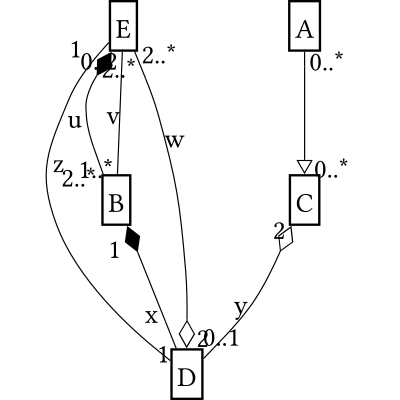
\includegraphics[min width=0.4\textwidth=0.6\textwidth,min height=0.4\textwidth=0.6\textwidth,keepaspectratio,max width=0.9\textwidth,max height=0.9\textwidth]{54/cdf0c034ae2b2d873c2c8affabc7eea3fa50026d3c82dac65b2adc16b689fafc6a01af83b04c596701db35357ce8aed00a3a92e08161.pdf}\end{centering}



It contains the following relationships between classes:

\begin{enumerate}\item[ 1 ]{composition x}
\item[ 2 ]{aggregation w}
\item[ 3 ]{aggregation y}
\item[ 4 ]{composition u}
\item[ 5 ]{the inheritance where A inherits from C and which has denoted the multiplicity 0..* near A and 0..* near C}
\item[ 6 ]{association z}
\item[ 7 ]{association v}
\end{enumerate}

Choose what you think is the single reason that this class diagram is incorrect, and mention all relationships that definitely contribute to the problem, i.e., removing any of them would fix the problem.

Reasons available to choose from are:

The class diagram ...

\begin{enumerate}\item[ a ]{contains at least two non-inheritance relationships between the same two classes pointing in opposite directions.}
\item[ b ]{contains at least one pair of classes each inheriting from the other.}
\item[ c ]{contains at least one self-inheritance.}
\item[ d ]{contains at least one inheritance cycle.}
\item[ e ]{contains at least one invalid multiplicity near the whole of a composition.}
\item[ f ]{contains at least one self-relationship that is no inheritance.}
\item[ g ]{contains at least one invalid multiplicity at some inheritance.}
\item[ h ]{contains at least one composition cycle.}
\item[ i ]{contains at least one multiple inheritance.}
\item[ j ]{contains at least two non-inheritance relationships between the same two classes.}
\end{enumerate}

Please state your answer by providing a letter for the reason, indicating the most specifically expressed reason for which you think this class diagram is invalid, and a listing of numbers for those relationships on whose individual presence the problem depends. For example,


\begin{minted}{text}
due-to:
- 3
- 4
reason: b

\end{minted}


would indicate that the class diagram is invalid because of reason b and that the 3. and 4. relationship (appearing together) create the problem.



Please note: Classes are represented simplified here. 
 That means they consist of a single box containing only the class name but no sections for attributes or methods. 
 Nevertheless you should treat these simplified class representations as valid classes.

Please note: When hovering over or clicking on edges / nodes or their labels, the respective components that belong together are highlighted.

